\documentclass{beamer}
\beamertemplatenavigationsymbolsempty
\usetheme{CambridgeUS}
\begin{document}
\title{2018 PbPb run MB Trigger Studies}
\subtitle{Day 1 Tasks}

%Slide 1
\begin{frame}
\frametitle{All ADC Distribution for Empty Bunches and ZB data}


\begin{figure}
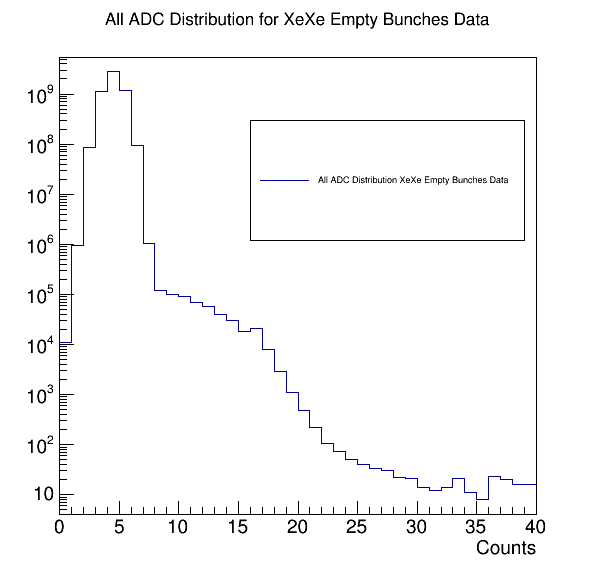
\includegraphics[width=0.38\textwidth]{Plots/AllEMBXADCDisLog.png}
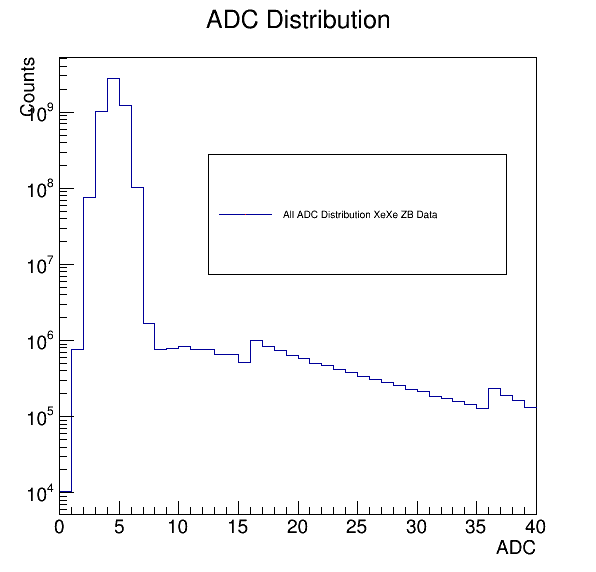
\includegraphics[width=0.38\textwidth]{Plots/AllZBADCDisLog.png}
\end{figure}

\begin{block}
{Comment: The left is XeXe empty bunches samples and the right is XeXe zero bias sample for all ADC distribution. Both of them ate plotted in log scale. We can see that both of the distribution has a peak near ADC = 5, which is the noise.}
\end{block}

\end{frame}

%Slide 2
\begin{frame}
\frametitle{Max ADC Distribution for Empty Bunches and ZB data}

\begin{figure}
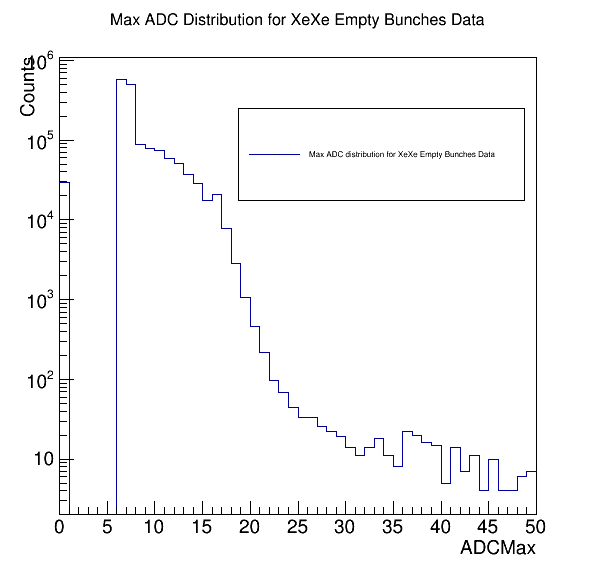
\includegraphics[width=0.38\textwidth]{Plots/ADCMaxEMBXLog.png}
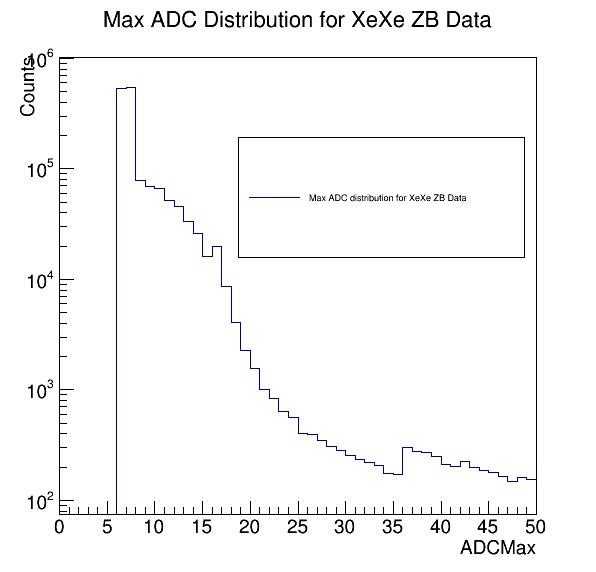
\includegraphics[width=0.38\textwidth]{Plots/ADCMaxZBLog.png}
\end{figure}

\begin{block}
{Comment: The left is XeXe empty bunches samples and the right is XeXe zero bias sample for max ADC distribution. Both of them ate plotted in log scale. We can see that both of the distribution starts at ADC = 5 and then decrease. Also, there are two bumps near ADC = 16 and ADC = 35 due to the different of ADC - HF energy conversion factors}
\end{block}
\end{frame}

%Slide 3

\begin{frame}
\frametitle{Max ADC and All ADC Distribution for Empty Bunches and ZB data plotted together}

\begin{figure}
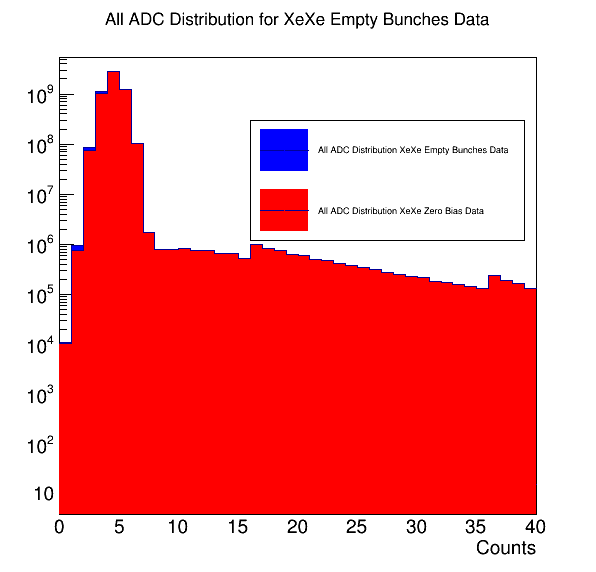
\includegraphics[width=0.38\textwidth]{Plots/AllBothADCDisLog.png}
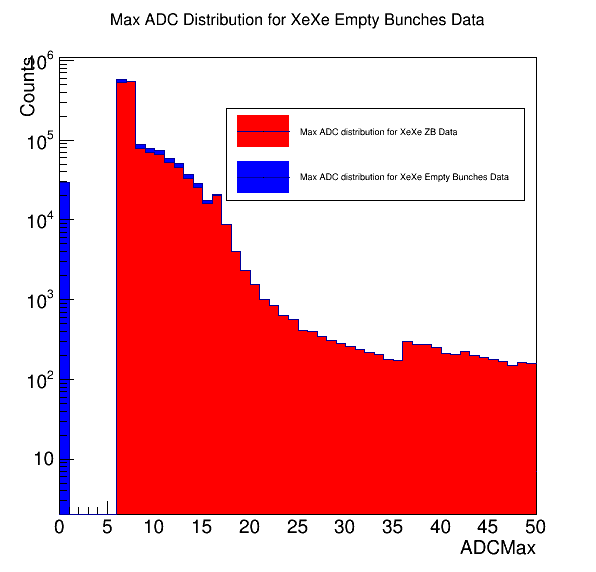
\includegraphics[width=0.38\textwidth]{Plots/ADCMaxBothLog.png}
\end{figure}

\begin{block}
{Comment: The left is all ADC distribution and the right plot is max ADC distribution. Both of them ate plotted in log scale. Empty bunches is in blue and zero bias is in red.}
\end{block}
\end{frame}


%Slide 4

\begin{frame}
\frametitle{MB OR and AND Trigger Efficiency vs ADC Thresholds}

\begin{figure}
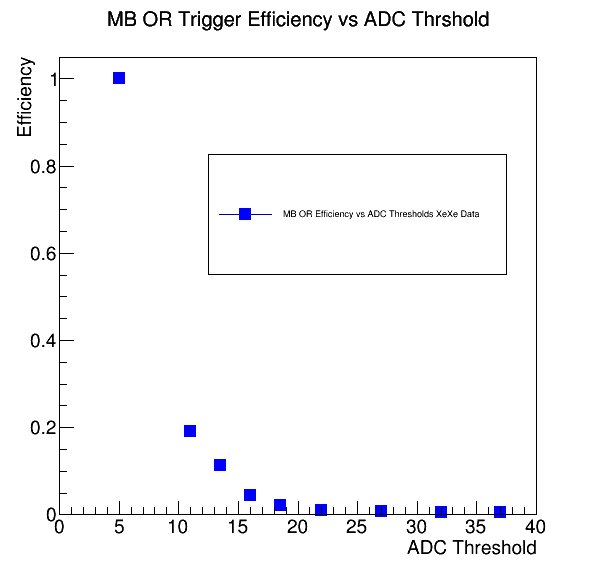
\includegraphics[width=0.38\textwidth]{Plots/MBOREfficiency.png}
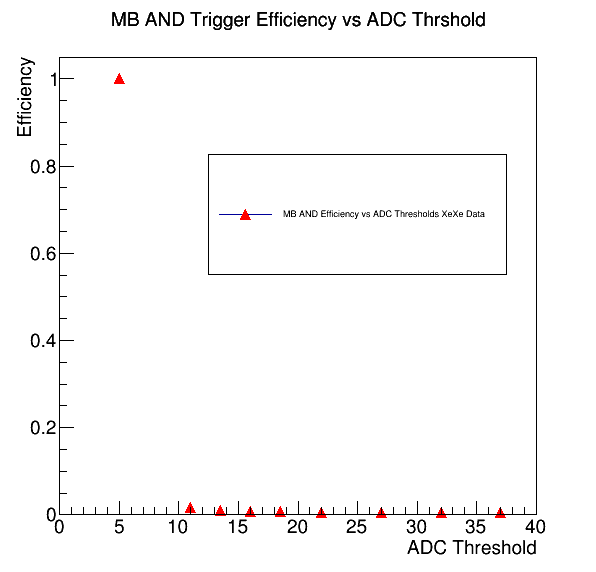
\includegraphics[width=0.38\textwidth]{Plots/MBANDEfficiency}
\end{figure}

\begin{block}
{Comment: The left is the MB OR trigger efficiency vs ADC thresholds and the right is MB AND efficiency for ADC thresholds. The trigger type is a standard trigger requiring any ADC readout to be greater than the ADC threshold in order to trigger an event. The data sample is zero bias.}
\end{block}
\end{frame}

%Slide 5

\begin{frame}
\frametitle{MB OR and AND Trigger Efficiency vs ADC Thresholds Plotted Together}

\begin{figure}
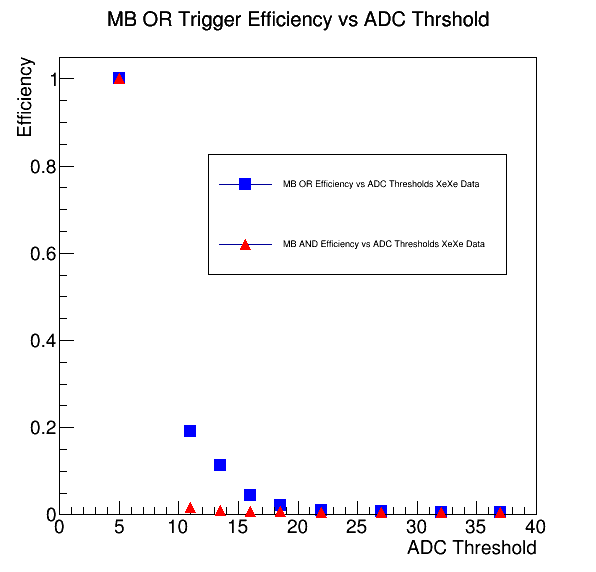
\includegraphics[width=0.38\textwidth]{Plots/MBEfficiencyBoth.png}

\end{figure}

\begin{block}
{Comment: The plot above is the MB trigger efficiency for both AND and OR plotted together. The OR trigger is in blue and the AND trigger is in red. We can see that the AND trigger is less efficient as OR since it require both forward and backward ADC to be greater than the ADC thresholds.}
\end{block}
\end{frame}

\end{document}